\documentclass[presentation]{beamer}
\usetheme{metropolis}
\titlegraphic{\hfill\includegraphics[height=2em]{imperial-bw-gray}}

\setbeamertemplate{bibliography item}{}
\setbeamertemplate{frametitle continuation}{%
  \usebeamerfont{frametitle}
  \uppercase\expandafter{\romannumeral \insertcontinuationcount\relax}
}

\metroset{progressbar=frametitle}

\graphicspath{{./\jobname.figures/}}

\usepackage{appendixnumberbeamer}

\usepackage{amsmath}
\usepackage{cancel}
\usepackage{pifont}
\newcommand{\cmark}{\ding{51}}
\newcommand{\xmark}{\ding{55}}

\usepackage{multirow}
\usepackage{bigdelim}
\usepackage[url=false,
doi=true,
isbn=false,
style=authoryear,
firstinits=true,
uniquename=init,
backend=biber]{biblatex}

\renewcommand{\bibfont}{\footnotesize}
\setlength{\bibitemsep}{1ex}
\renewbibmacro{in:}{}
\DeclareFieldFormat[article]{volume}{\textbf{#1}}
\DeclareFieldFormat{doi}{%
  doi\addcolon%
  {\scriptsize\ifhyperref{\href{http://dx.doi.org/#1}{\nolinkurl{#1}}}
    {\nolinkurl{#1}}}}
\AtEveryBibitem{%
\clearfield{pages}%
\clearfield{issue}%
\clearfield{number}%
}

\addbibresource{../literature.bib}

\title{From here to there}
\subtitle{challenges for \cancel{peta} exa-scale transient simulation}
\date{27th March 2017}

\author{Lawrence Mitchell\inst{1,*}}
\institute{
\inst{1}Departments of Computing and Mathematics, Imperial College
London

\inst{*}\texttt{lawrence.mitchell@imperial.ac.uk}
}

\begin{document}

\maketitle

\section{What do we want?}

\begin{frame}[standout]
  50GHz single-core CPUs
\end{frame}

\section{What do we have?}

\begin{frame}
  \frametitle{Too many cores}
  {\small
  \begin{tabular}{lccccc}
    Chip & Cores & TF/s & GB/s & F/B & Power \\
    \hline
    NVidia P100 & 56 (3584) & 5.3 & 730 & 7.2 & 250 (21 GF/W) \\
    Xeon Phi 7290F & 72 & 3.5 & 450 + 100 & 5.4 & 260 (13 GF/W) \\
    Broadwell & 22 & 0.78 & 150 & 5.2 & 140 (5.6 GF/W)
  \end{tabular}
  }

  \begin{block}{Exascale}
    \begin{itemize}
    \item<1-> 190K NVidia P100s, 1e9-way concurrency, 150MW
    \item<1-> 290K Intel Phis, 1e8-way concurrency, 220MW
    \item<1-> 1.3M Intel Broadwells, 3e7-way concurrency, 540MW
    \item<2-> 1 Boeing 747, 140MW
    \item<3-> 1 Google, 650MW
    \item<4-> 1 Sizewell B, 1200MW
    \item<5-> 1 UK, 35GW
    \end{itemize}
  \end{block}
\end{frame}

\begin{frame}
  \frametitle{What's happened to the chips}
  \begin{itemize}
  \item Number of transistors still increasing exponentially
  \item Frequency flat since c.~2005
  \item Performance through on-chip parallelism: ``now it's your
    problem''
  \item Wider ``atomic'' floating point instructions
  \end{itemize}

  \begin{tabular}{lcccc}
    Chip           & Cores & Clock & Vector width & Historical proxy         \\
    \hline
    P100           & 56    & 1.5   & 32           & CM-1                     \\
    Broadwell      & 22    & 2.2   & 4            & \multirow{4}{*}{Cray X1} \\
    Phi            & 72    & 1.5   & 8            &                          \\
    Skylake        & 32    & 2.2   & 8            &                          \\
    ARMv8 (Cavium) & 54?   & 2?    & 4-32?        &                          \\
  \end{tabular}
\end{frame}

\section{What should we do?}

\begin{frame}[standout]
 Run LINPACK
\end{frame}

\begin{frame}
  \frametitle{But seriously}
  \begin{itemize}
  \item High arithmetic intensity (flops are cheaper than bytes)
  \item Vectorise, vectorise, vectorise (only way to achieve flops)
  \item Avoid bulk synchronous computation (performance resilience)
  \item Reduce and/or amortise communication (hide latency)
  \end{itemize}
\end{frame}

\begin{frame}
  \frametitle{The status quo}
  \begin{itemize}
  \item[\xmark] Low order, memory bound
  \item[\xmark] Vectorisation left to compiler (?)
  \item[\xmark] Iterative schemes with blocking reductions
  \item[\xmark] Simple communication patterns (not optimal?)
  \end{itemize}
\end{frame}


\section{What to look for}

\begin{frame}
  \frametitle{Algorithmic optimality}
  \begin{block}{Notation}
  $N$ -- total number of degrees of freedom;

  $P$ -- total number of processes;

  $T(N, P)$ -- time to solution.
  \end{block}

  \begin{block}{Desired}
    $\mathcal{O}(N)$ computational complexity;

    $\mathcal{O}(\log P)$ communication complexity.

    Be aware of the constants!
  \end{block}
\end{frame}

\begin{frame}
  \frametitle{Parallel scalability}

  \begin{block}{Weak scaling}
    Constant local work $N/P$.

    Scalable code has $T(N, P) = T(2N, 2P)$.
  \end{block}

  \begin{block}{Strong scaling}
    Decreasing local work $N/P$.

    Scalable code has $T(N, P) = 2T(N, 2P)$.
  \end{block}

\end{frame}

\begin{frame}
  \frametitle{Transient simulation}
  {\large
    Time-resolved transient simulations do not weak scale. Sad!
  }

  \begin{block}{What to do?}
    \begin{itemize}
    \item Get algorithmics right
    \item Work hard to attack constant factors
    \item Work on strong scaling efficiency
    \item Develop \emph{predictive} models of performance to
      \emph{understand} why codes behave how they do.
    \end{itemize}
  \end{block}

\end{frame}

\begin{frame}
  \frametitle{Predicting scalability}

  Summarising \textcite{Fischer:2015}.
  
  \begin{block}{Notation}
    \begin{itemize}
    \item parallelisable work: $T_a(N, P) = T_a(N, 1)/P$

    \item communication: $T_c(N, P)$

    \item serial overhead: $c \approx 0$

    \item time to solution
      \begin{equation*}
        T(N, P) = \left\{
          \begin{aligned}
            &T_a(N, P) + T_c(N, P) + c &\text{ synchronous}\\
            &\max(T_a(N, P), T_c(N, P)) + c\,\,&\text{ asynchronous}
          \end{aligned}\right.
      \end{equation*}

    \item scaling efficiency: $\eta = \frac{T(N, 1)}{PT(N,P)}$
  \end{itemize}
  \end{block}
\end{frame}

\begin{frame}
  \frametitle{When to stop adding cores?}

  \begin{block}{Minimum $T(N, P)$}
    Find $P$ such that $\frac{\text{d} T(N, P)}{\text{d} P} = 0$.

    Typically too expensive (wasting many core hours).
  \end{block}

  \begin{block}{A compromise}
    Find $P$ such that $T_a(N, P) = T_c(N, P)$, $\eta = 0.5$ for
    synchronous case.
  \end{block}

  \begin{theorem}[Anonymous]
    Krylov methods strong scale to $N/P \approx 30000$.

    Explicit schemes are a little better $N/P \approx 10000$.

    ``Reductions limit scalability''
  \end{theorem}
\end{frame}

\begin{frame}
  \frametitle{Empirical scaling limits}
  
  \begin{itemize}
  \item Measure $T(N, P_\text{min})$ and $T(N, P)$ for a range of
    process counts.

  \item Pick $P_\text{opt}$ such that
    $P_\text{opt}T(N, P_\text{opt}) = 2T(N,P_\text{min})$.

  \item How do I know if that is any good?
  \end{itemize}
\end{frame}

\begin{frame}
  \frametitle{Building blocks}
  \begin{block}{Computation}
    Measure $S$, e.g., flops with $P=1$, $N$ large.

    ``atomic'' unit of computation takes time $t_a = S^{-1}$.
  \end{block}

  \begin{block}{Communication}
    Linear model, latency + bandwidth.

    Time (s) to send $m$ doubles
    \begin{equation*}
      t_c(m) = \alpha^* + \beta^* m
    \end{equation*}
    non-dimensionalise, $\alpha = \alpha^*/t_a$, $\beta =
    \beta^*/t_a$.
    \begin{equation*}
      t_c(m) = (\alpha + \beta m)t_a
    \end{equation*}
  \end{block}
\end{frame}

\begin{frame}
  \frametitle{Run some measurements}
  \begin{center}
    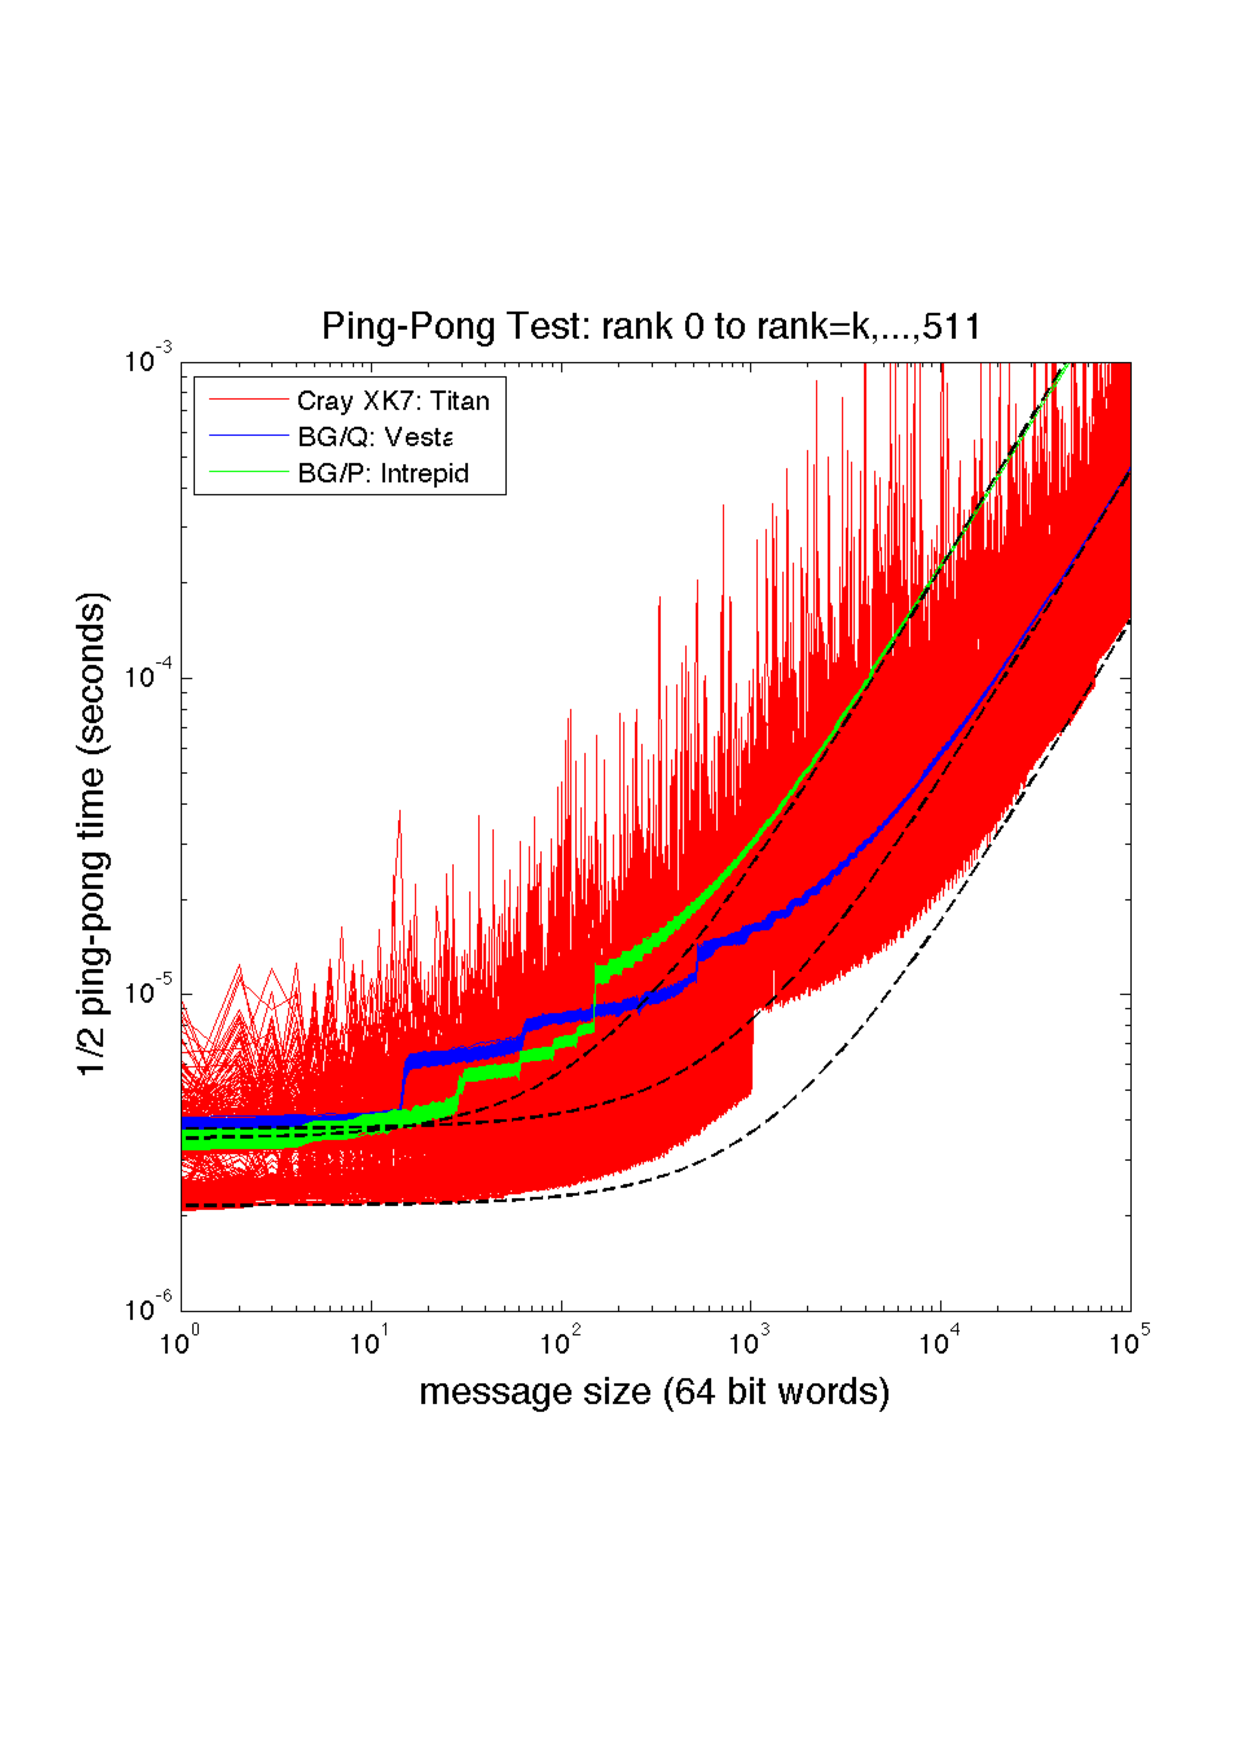
\includegraphics[height=0.8\textheight]{ping-pong}
  \end{center}
  From \textcite{Fischer:2015}.
\end{frame}

\begin{frame}
  \frametitle{Performance variability}
  \begin{itemize}
  \item Model is pretty good
  \item Network topology + load can affect even simple codes
  \item BlueGene has torus network, each job gets a convex subset
  \item Not true on Cray (Dragonfly), network traffic
    from other jobs can affect your performance \parencite{Prisacari:2014}.
  \end{itemize}
\end{frame}

\begin{frame}
  \frametitle{Jacobi iteration, 7-point 3D stencil}
  \begin{equation*}
    u_i^{k+1} = a_{ii}^{-1}\left(f_i + \sum_{j \ne i} a_{ij}u_j^{k}\right)
  \end{equation*}
  counting operations with $N/P$ entries per process.
  \begin{equation*}
    T_a = 14(N/P)t_a.
  \end{equation*}
  With a block decomposition, each face exchange moves $(N/P)^{2/3}$
  values, so
  \begin{equation*}
    T_c = 6 \left(\alpha + \beta (N/P)^{2/3}\right)t_a.
  \end{equation*}

  With $\alpha = 3750, \beta = 2.86$ (BG/Q), $T_a = T_c$ when $N/P
  \approx 1700$.  \emph{Independent} of $P$.

  If $\beta = 0$, $N/P \approx 1600$.
\end{frame}


\begin{frame}
  \frametitle{Conjugate gradients, 7-point 3D stencil}
  \begin{equation*}
    T_a = 27(N/P) t_a
  \end{equation*}
  Again, we need 6 face exchanges, plus two reductions (each $2\alpha t_a \log_2 P$)
  \begin{equation*}
    T_c = 6 \left(\alpha + \beta (N/P)^{2/3}\right)t_a + 2 \cdot 2
    \alpha t_a \log_2 P.
  \end{equation*}

  Now the scaling limit is $P$-dependent.

  \begin{itemize}
    \item $P=10^6$: $N/P \approx 12000$;
    \item $P=10^9$: $N/P \approx 17000$.
  \end{itemize}
\end{frame}

\begin{frame}
  \frametitle{But wait}
  \begin{columns}
    \begin{column}{0.6\textwidth}
      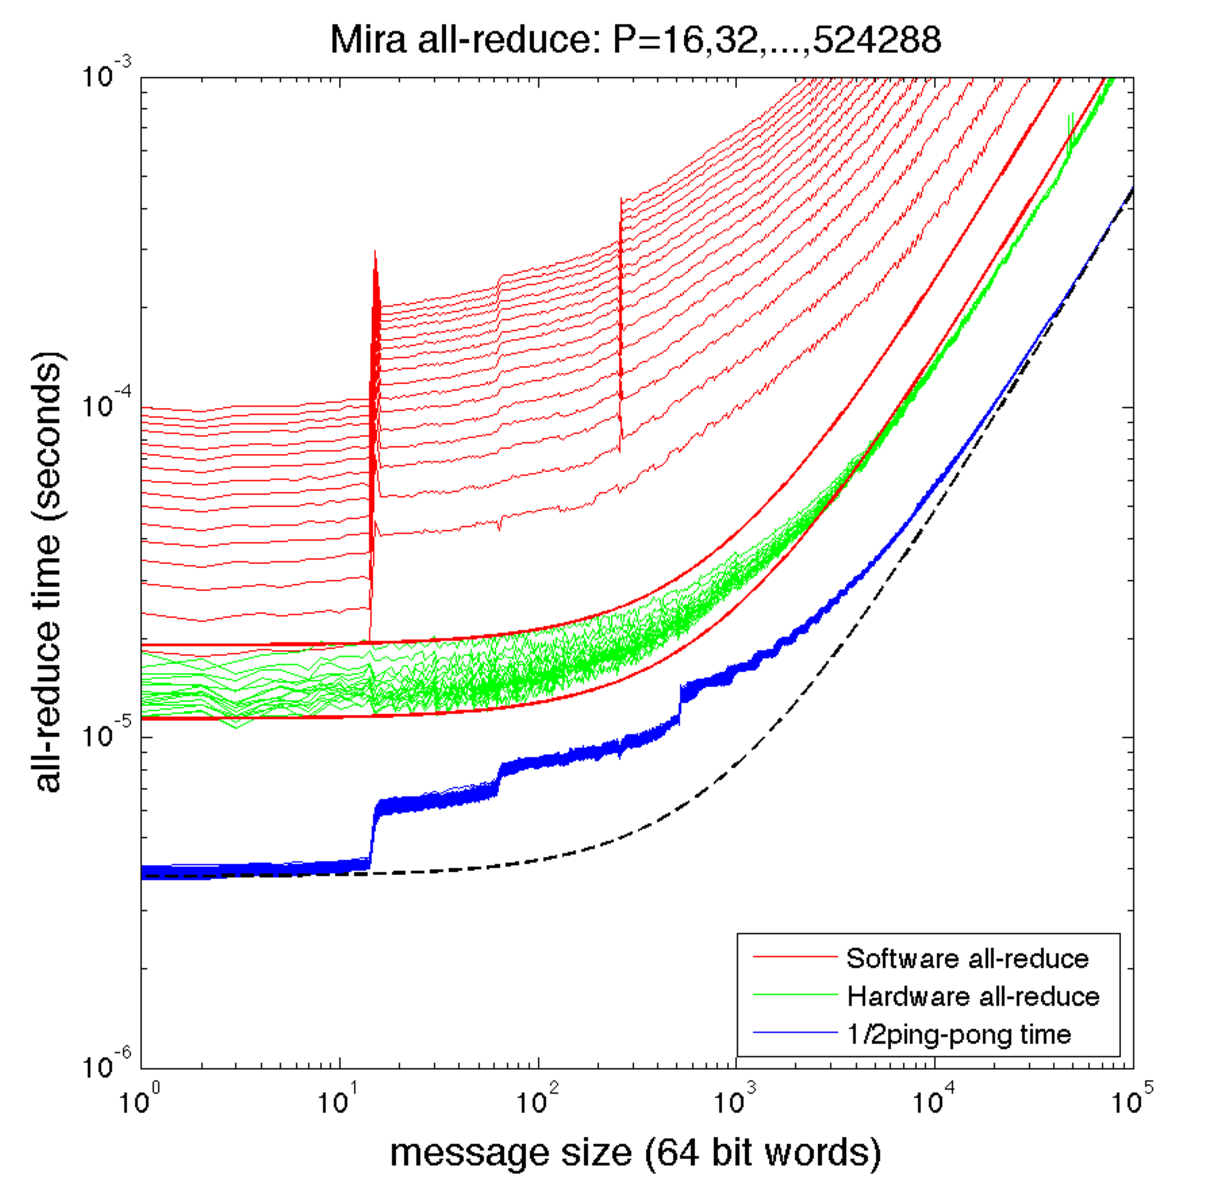
\includegraphics[width=\columnwidth]{allreduce}

      From \textcite{Fischer:2015}.
    \end{column}
    \begin{column}{0.4\textwidth}
      \begin{itemize}
      \item Hardware-level allreduce on BlueGene is \emph{$P$
          independent}.
      \item On the full machine, a reduction costs $5\alpha$.
      \end{itemize}
    \end{column}
  \end{columns}
\end{frame}

\begin{frame}
  \frametitle{Round again}
  \begin{equation*}
    T_c = 6 \left(\alpha + \beta (N/P)^{2/3}\right)t_a +
    \cancel{2\cdot 2 \log_2 P \alpha t_a} + 2 \cdot 5 \alpha t_a.
  \end{equation*}

  Now we have $P$-\emph{independent} scaling behaviour, $N/P \approx 2100$.

  Using only a single reduction, we can get to $N/P \approx
  1500$.

  8x more strong scaling on $P=10^9$, with no increase in
  power consumption.

  A similar analysis can be done for multilevel algorithms,
  e.g.~for Poisson $N/P \approx 10000$ (constant reduction complexity).
\end{frame}

\begin{frame}
  \frametitle{Some data points}

  \begin{onlyenv}<1>
    3-D incompressible Navier-Stokes for reactor cooling, NEK5000.
    High order, spectral element.  60\% time in multigrid Poisson solves.

    \begin{center}
      \includegraphics[height=0.6\textheight]{nek-strong-scale}

      Data reproduced from \textcite{Fischer:2015}.
    \end{center}
  \end{onlyenv}

  \begin{onlyenv}<2>
    3-D non-hydrostatic baroclinic instability 3km resolution, Gordon Bell prize
    2016.  Low order, finite volume. Most time in multigrid Helmholtz solve.
    \begin{center}
      \includegraphics[height=0.6\textheight]{sunway-strong-scale}

      Data reproduced from \textcite{Yang:2016}.
    \end{center}
  \end{onlyenv}

  \begin{onlyenv}<3>
    3-D nonlinear Stokes for mantle convection, Gordon Bell prize
    2015.  High order, finite element.  Time split between viscous
    and pressure-Poisson multigrid solves.

    \begin{center}
      \includegraphics[height=0.6\textheight]{mantle-strong-scale}

      Data reproduced from \textcite{Rudi:2015}.
    \end{center}    
  \end{onlyenv}
\end{frame}

\begin{frame}
  \frametitle{Latency hurts}

  \begin{itemize}
  \item When strong-scaling mesh codes, you don't care about network
    bandwidth.
  \item Decreasing $\alpha$ is important, pester your vendor!
  \item Faster cores (relative to network) means worse strong scaling.
  \item Faster code means worse strong scaling.
  \end{itemize}
\end{frame}

\begin{frame}
  \frametitle{Some thoughts on climate codes}

  \begin{block}{Conjecture}
    Operational climate models make nowhere near optimal use of current
    hardware.

    Extrapolating current SYPD to larger problems is perhaps not
    useful, unless we think the current models are good.
  \end{block}

  \begin{itemize}
  \item More work means scaling should improve.
  \item Will column-wise data decomposition start to hurt?
  \item Lobby for power spend on interconnect, not cores?
  \item Don't forget to focus on minimising time-to-solution first.
  \end{itemize}
\end{frame}

\section{What might we do?}

\begin{frame}
  \frametitle{Improving SYPD}

  \begin{itemize}
  \item Better serial performance.  Is it the case that current codes
    make efficient use of hardware?

  \item High order?  Only useful if we can use fewer dofs.  Are models in
    the asymptotic region where we expect exponential accuracy gains
    from high order discretisations?

  \item Better strong scaling.  Necessary to counteract timestep
    restrictions with increasing resolution.
  \end{itemize}
\end{frame}

\begin{frame}
  \frametitle{Better serial performance}

  \begin{itemize}
  \item Ground up rewrites of models?

  \item Optimising ``line by line'' doesn't work, we're stuck
    in local minima.  e.g.~changes in data layout require a large
    scale changes if the data model is implicit.
  
  \item Look for opportunities to reduce algorithmic complexities

  \item \textcite{Yang:2016} and \textcite{Rudi:2015} are examples of
    what you can do for single components.
  \end{itemize}
\end{frame}

\begin{frame}
  \frametitle{High order?}
  \begin{itemize}
  \item High order, flop heavy, schemes are more suited to modern
    architectures
  \item But often not in asymptotic convergence region
  \item Need to have competitive performance \emph{per dof}
  \item FE probably preferable to FV or FD, since minimal stencil (less comms).
  \end{itemize}
\end{frame}
\begin{frame}
  \frametitle{Addressing latency}

  \begin{itemize}
  \item Reducing $\alpha$ has a big effect on scaling limits
  \item $\alpha \rightarrow \alpha/10$ would allow scaling Poisson
    multigrid to $N/P\approx 900$.  \alert{10x} in time to solution
    for same power.
  \item Similarly, hardware reductions are \emph{really} important.
  \item Would we be happy if vendors spent more of the power budget on
    network and less on chips?
  \end{itemize}
\end{frame}

\begin{frame}
  \frametitle{Reducing communication}

  \begin{block}{$\tau$-FAS}
    \begin{itemize}
    \item $\tau$ formulation of multigrid (\textcite{Brandt:1977},
      \textcite[\S 8.3]{Brandt:2011}) admits low data transfer
      implementation \parencite{Brandt:1994}.

    \item Performance modelling and results for 27 point FV Poisson
      problem in \textcite{Adams:2016}.

    \item Worthwhile to try if you already have a FAS for your problem?
    \end{itemize}
  \end{block}
\end{frame}

\begin{frame}
  \frametitle{Tiling to amortise latency}
  \begin{itemize}
  \item  \emph{Diamond tiling} is a well known optimisation in computer
    science for stencil codes.

    \begin{center}
      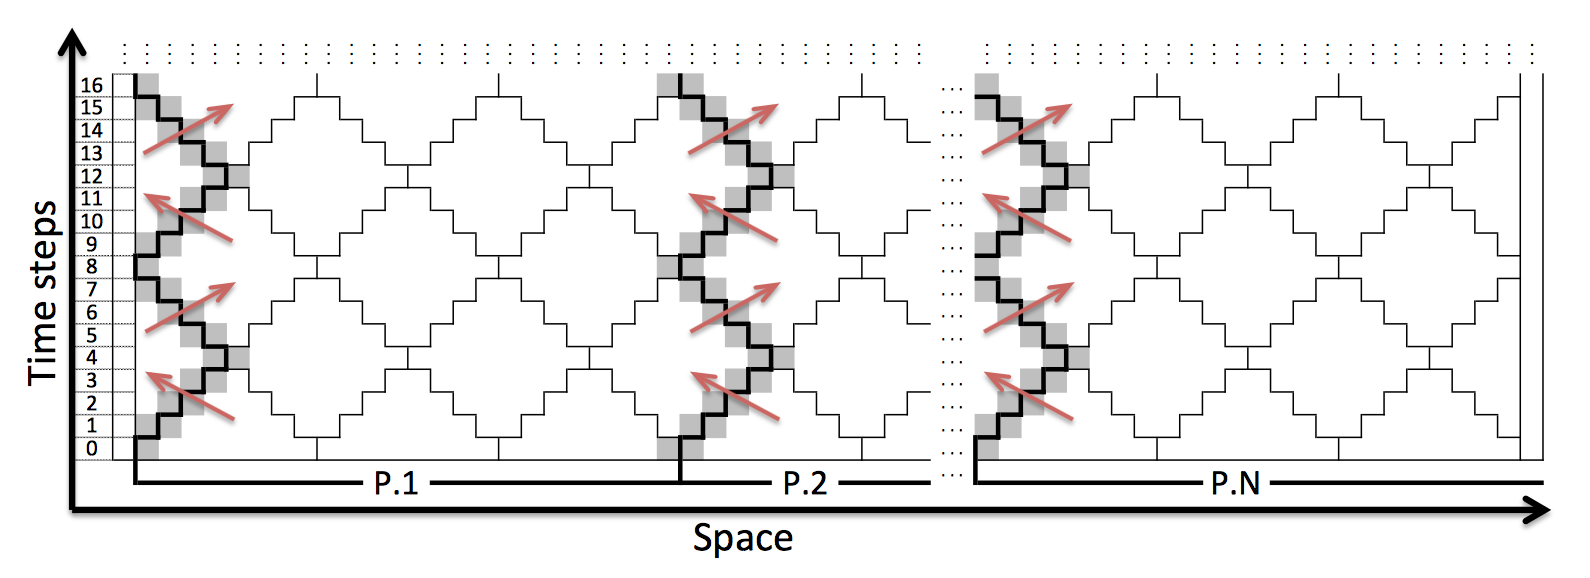
\includegraphics[width=0.7\textwidth]{diamond-mpi}
    \end{center}
  \item Typically used for better cache usage.
  \item Can be extended to hide network latency.
  \item Good analysis in \textcite{Malas:2015}
  \item ``Rediscovered'' in \textcite{Alhubail:2016}.
  \item Explicit schemes only.
  \end{itemize}
\end{frame}

\begin{frame}[t]
  \frametitle{Asynchronous algorithms}
  \begin{itemize}
  \item Harden against OS jitter by removing barriers
  \item Hide latency
  \item Potential for soft error recovery
  \item Is MTTF \emph{really} a problem?  The same things were being
    warned of petascale systems.
  \end{itemize}

  \begin{onlyenv}<2>
    \begin{block}{Pipelined Krylov methods}
      \begin{itemize}
      \item Use asynchronous reductions \textcite{Ghysels:2013a}.
      \item Not aware of any group other than Vanroose's that shows
        such performance improvements.
      \item Best suited to simple preconditioners.
      \end{itemize}
    \end{block}
  \end{onlyenv}

  \begin{onlyenv}<3>
    \begin{block}{$s$-step Krylov methods}
      \begin{itemize}
      \item AKA communication avoiding Krylov.
      \item Mostly work from Demmel's group.
      \item Again, don't work with ``good'' preconditioners.
      \item Erin Carson's thesis \parencite{Carson:2015} is an
        excellent, and honest, summary of the current state.
      \end{itemize}
    \end{block}
  \end{onlyenv}
\end{frame}

\begin{frame}
  \frametitle{Is time parallel the answer?}
  \begin{itemize}
  \item At some point, traditional timestepping will stop scaling
  \item Time parallel is perhaps a way around this
  \item Need to be honest.  Can we get speedups relative to the best
    ``traditional'' model?
  \item Are we better off running bigger ensembles?  Better data
    assimilation?
  \end{itemize}
\end{frame}

\begin{frame}[standout]
  Questions?
\end{frame}

\appendix

\begin{frame}[allowframebreaks]
  \frametitle{References}
  
  \printbibliography[heading=none]
\end{frame}
\end{document}
